%=======================================================
% CHAPTER 3: HARD PROBLEMS
%=======================================================

\begin{frame}[plain]
  \begin{center}\bfseries\centering
    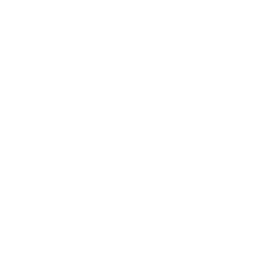
\includegraphics[scale=1]{assets/branding/opa0}
    \vspace{-5.75cm}\\
    {\adjustbox{scale=1.95}{\color{TealDarkCyan}\;IV.\;Hard Problems}}
    \vspace{.25cm}
    \begin{minipage}{.78\textwidth}
      \scriptsize\color{Ink}
      \textbf{Big picture.}\; Hardness comes from the gap between an easy basis description and hard geometric search.\\[.2cm]
      \textbf{Details to watch.}\; SVP, CVP, BDD, SIVP, GapSVP, LLL, and approximation factors.
    \end{minipage}
    {\ }\vspace{2.1cm}\\
    \bigskip
  \end{center}
\end{frame}

\begin{frame}[shrink=5]{\textbf{IV. Hard Problems}}{SVP}
\defbox[Shortest Vector Problem]{
Given a basis $\mat B$ of a lattice $\Lat$, find a nonzero vector $v\in\Lat$ such that
\[
  \norm v=\lambda_1(\Lat).
\]
}
\begin{columns}[T,onlytextwidth]
\begin{column}{.50\textwidth}
\textcolor{TealDarkCyan}{\textbf{Approximate SVP}}
\[
  \norm v\le \gamma(n)\lambda_1(\Lat).
\]
\begin{itemize}
  \item Exact SVP is too strong for many applications.
  \item Approximation factors encode the security target.
\end{itemize}
\end{column}
\begin{column}{.46\textwidth}
\textcolor{TealDarkCyan}{\textbf{Basis trap}}
\begin{itemize}
  \item A basis vector may be exponentially longer than $\lambda_1$.
  \item Short combinations can have large integer coefficients in a bad basis.
\end{itemize}
\end{column}
\end{columns}
\textbf{Toy instance.}\; For $\Lat=2\Z\times5\Z$, SVP returns $(\pm2,0)$ and $\lambda_1=2$.
With $c_1=(1001,1000)$, $c_2=(1000,999)$, the short vector is hidden as $c_1-c_2=(1,1)$.
\end{frame}

\begin{frame}[shrink=5]{\textbf{IV. Hard Problems}}{CVP}
\defbox[Closest Vector Problem]{
Given a basis of $\Lat\subset\R^n$ and a target $t\in\R^n$, find $v\in\Lat$ minimizing
\[
  \norm{t-v}.
\]
}
\begin{columns}[T,onlytextwidth]
\begin{column}{.52\textwidth}
\begin{itemize}
  \item CVP asks for the lattice point in the same Voronoi cell as $t$.
  \item Bounded Distance Decoding (BDD) is CVP with a promise that $t$ is close to the lattice.
  \item Decoding linear codes and decoding lattices are parallel ideas.
\end{itemize}
\textbf{Example in $\Z^2$.}\; For $t=(2.2,4.7)$, the closest point is $(2,5)$.
For a skew lattice, nearest-point search is no longer coordinate-wise rounding.
\end{column}
\begin{column}{.43\textwidth}
\begin{center}
\begin{tikzpicture}[scale=.62]
  \clip (-3,-2.6) rectangle (3.3,2.8);
  \foreach \i in {-4,...,4}{
    \foreach \j in {-4,...,4}{
      \node[lattice point] at ({\i+0.48*\j},{0.78*\j}) {};
    }
  }
  \coordinate (t) at (1.22,.52);
  \node[circle,fill=ErrorRed,inner sep=2pt,label=right:$t$] at (t) {};
  \draw[flow red] (t) -- (1,0) node[midway,right,tiny label] {error};
  \draw[ErrorRed!35,line width=.8pt] (1,0) circle (.78);
  \node[caption text] at (0,-2.15) {closest lattice point to a target};
\end{tikzpicture}
\end{center}
\end{column}
\end{columns}
\end{frame}

\begin{frame}[shrink=8]{\textbf{IV. Hard Problems}}{SIVP and GapSVP}
\begin{columns}[T,onlytextwidth]
\begin{column}{.48\textwidth}
\defbox[SIVP]{
Given a basis of $\Lat$, find $n$ linearly independent vectors
\[
  v_1,\ldots,v_n\in\Lat
\]
with $\max_i\norm{v_i}\le \gamma(n)\lambda_n(\Lat)$.
}
\end{column}
\begin{column}{.48\textwidth}
\defbox[GapSVP]{
Given a threshold $d$, distinguish between
\[
  \lambda_1(\Lat)\le d
  \quad\text{and}\quad
  \lambda_1(\Lat)>\gamma(n)d.
\]
}
\end{column}
\end{columns}
\bigskip
\textcolor{TealDarkCyan}{\textbf{Why they appear in reductions}}
\begin{itemize}
  \item SIVP captures the need for many independent short directions.
  \item GapSVP turns search geometry into a decision problem.
  \item Worst-case reductions often target approximate versions of these problems.
\end{itemize}
\textbf{Example.}\; For $\Lat=2\Z\times5\Z$, SIVP needs $(2,0)$ and $(0,5)$.
GapSVP with $d=3$ and $\gamma=2$ asks whether $\lambda_1\le3$ or $\lambda_1>6$.
\end{frame}

\begin{frame}[shrink=5]{\textbf{IV. Hard Problems}}{Naive Algorithms}
\textcolor{TealDarkCyan}{\textbf{Enumeration}}
\begin{itemize}
  \item Search all integer vectors $z$ with $\norm{\mat Bz}\le R$.
  \item Works in low dimensions.
  \item The search tree grows exponentially with the dimension.
\end{itemize}
\bigskip
\textcolor{TealDarkCyan}{\textbf{Voronoi methods}}
\begin{itemize}
  \item Describe the Voronoi cell and use its facets.
  \item Exact but exponential.
\end{itemize}
\bigskip
\textbf{\color{red}Lesson.}\; Exact lattice problems are feasible for small $n$ and become rapidly expensive.
\textbf{Enumeration scale.}\; If $z_i\in[-10,10]$, brute force checks $21^n$ candidates:
$441$ in dimension $2$, but about $1.7\times10^{13}$ in dimension $10$.
\end{frame}

\begin{frame}{\textbf{IV. Hard Problems}}{Visualization: Enumeration Explosion}
\small
\begin{columns}[T,onlytextwidth]
\begin{column}{.43\textwidth}
\textbf{Coefficient search.}\; Enumeration searches integer coordinates first:
\[
  z=(z_1,\ldots,z_n),\qquad \norm{\mat Bz}\le R.
\]
If each coordinate has $2R+1$ choices, the raw search width is
\[
  (2R+1)^n.
\]
\textbf{The geometry filters candidates, but the tree is still exponential.}
\end{column}
\begin{column}{.53\textwidth}
\begin{center}
\begin{tikzpicture}[scale=.72]
  \node[process] (root) at (0,1.8) {$z_1$};
  \foreach \x/\lab [count=\k] in {-2/-1,0/0,2/1}{
    \node[process blue,minimum width=.8cm] (a\k) at (\x,.65) {$\lab$};
    \draw[flow] (root) -- (a\k);
    \foreach \d/\labtwo in {-.55/-1,0/0,.55/1}{
      \node[circle,draw=AmberCode!65,fill=AmberCode!10,inner sep=2.0pt] at ({\x+\d},-.55) {};
      \draw[flow amber] (a\k) -- ({\x+\d},-.55);
    }
  }
  \node[tiny label] at (-2.55,-.95) {$z_2=-1,0,1$};
  \node[tiny label] at (0,-1.35) {$3^2$ partial nodes};
  \node[process red,align=center] at (0,-2.25)
    {after $n$ levels:\\$(2R+1)^n$ candidates};
\end{tikzpicture}
\end{center}
\end{column}
\end{columns}
\end{frame}

\begin{frame}[shrink=8]{\textbf{IV. Hard Problems}}{LLL Reduction}
\defbox[Goal of basis reduction]{
Replace a bad basis by a better basis of the same lattice:
\[
  \mat B\longmapsto \mat B\mat U,\qquad \mat U\in\GL_n(\Z).
\]
}
\thmbox[LLL theorem, informal]{
The LLL algorithm runs in polynomial time and outputs a basis whose first vector satisfies
\[
  \norm{b_1}\le 2^{(n-1)/2}\lambda_1(\Lat).
\]
}
\begin{itemize}
  \item LLL is powerful in practice but gives an exponential approximation factor.
  \item Stronger block reduction algorithms trade more time for better quality.
  \item Lattice cryptography chooses parameters beyond known reduction attacks.
\end{itemize}
\textbf{Concrete effect.}\; Starting from $c_1=(1001,1000)$ and $c_2=(1000,999)$, integer subtraction exposes
\[
  c_1-c_2=(1,1).
\]
LLL automates this kind of basis improvement in high dimension.
\end{frame}

\begin{frame}{\textbf{IV. Hard Problems}}{Visualization: LLL Finds Integer Cancellations}
\small
\begin{columns}[T,onlytextwidth]
\begin{column}{.51\textwidth}
\begin{center}
\begin{tikzpicture}[scale=.68,transform shape]
  \useasboundingbox (-.45,-2.75) rectangle (3.85,2.65);
  \coordinate (O) at (0,0);
  \coordinate (C1) at (3.35,2.25);
  \coordinate (C2) at (3.05,1.95);
  \draw[basis vector] (O) -- (C1) node[above] {$c_1$};
  \draw[basis vector] (O) -- (C2) node[below right] {$c_2$};
  \draw[short vector] (C2) -- (C1) node[midway,right] {$c_1-c_2$};
  \draw[TealDarkCyan!35,dashed] (2.65,1.55) rectangle (3.65,2.55);
  \begin{scope}[shift={(.35,-1.55)},scale=1.35]
    \draw[panel] (-.25,-.25) rectangle (1.25,1.25);
    \draw[short vector] (0,0) -- (1,1) node[above right] {$(1,1)$};
    \node[tiny label] at (.55,-.18) {zoom};
  \end{scope}
  \node[caption text,align=center,text width=4.2cm] at (1.7,-2.45)
    {a very short vector can be a difference of long basis vectors};
\end{tikzpicture}
\end{center}
\end{column}
\begin{column}{.45\textwidth}
\[
  c_1=(1001,1000),\qquad c_2=(1000,999).
\]
\[
  c_1-c_2=(1,1).
\]
\textbf{What reduction does.}\; It repeatedly replaces a vector by an integer combination that exposes shorter directions in the same lattice.
\end{column}
\end{columns}
\end{frame}

\begin{frame}{\textbf{IV. Hard Problems}}{Penetrating Example: Subset Sum I}
\small
\defbox[Subset sum]{
Given weights $a_1,\ldots,a_n$ and target $T$, find $x\in\{0,1\}^n$ such that
\[
  \sum_{i=1}^n a_i x_i=T.
\]
}
\textbf{Lattice embedding.}\; For a large scale $M$, generate a lattice in $\R^{n+1}$ by
\[
  (e_i,\;Ma_i)\quad(1\le i\le n),\qquad (0,\ldots,0,\;-MT).
\]
If $x$ is a solution, the lattice contains
\[
  (x_1,\ldots,x_n,\;M(\sum a_i x_i-T))=(x_1,\ldots,x_n,0),
\]
which is unusually short.

\textbf{Why this is penetrating.}\; The combinatorial condition ``exactly hit $T$'' is converted into the geometric condition ``make the last coordinate zero.''  Large $M$ makes wrong sums visibly long.
\end{frame}

\begin{frame}{\textbf{IV. Hard Problems}}{Penetrating Example: Subset Sum II}
\small
\begin{columns}[T,onlytextwidth]
\begin{column}{.44\textwidth}
\textbf{Concrete instance.}
\[
\begin{array}{rcl}
a&=&(366,385,392,401,\\
 &&\quad 422,437,450,463),\\
T&=&1204.
\end{array}
\]
\[
  366+401+437=1204.
\]
So LLL is asked to find the short vector
\[
  (1,0,0,1,0,1,0,0,0).
\]
\end{column}
\begin{column}{.52\textwidth}
\textbf{What LLL sees.}\; The vector has length $\sqrt3$, while a wrong subset with sum error $r\ne0$ has last coordinate $Mr$.

\vspace{.4em}
For $M=100$, even a one-unit target miss contributes length at least $100$.
\end{column}
\end{columns}
\begin{center}
\begin{tikzpicture}[node distance=.66cm]
  \node[process] (comb) {combinatorial\\subset};
  \node[process blue, right=1.1cm of comb] (lat) {integer\\lattice};
  \node[process amber, right=1.1cm of lat] (short) {short\\$0/1$ vector};
  \node[process red, right=1.1cm of short] (sol) {subset\\solution};
  \draw[flow] (comb) -- node[above,tiny label] {embed} (lat);
  \draw[flow blue] (lat) -- node[above,tiny label] {LLL} (short);
  \draw[flow amber] (short) -- node[above,tiny label] {read support} (sol);
\end{tikzpicture}
\end{center}
\textbf{Point.}\; A discrete search problem becomes a geometric question: is the hidden $0/1$ vector among the shortest lattice vectors?
\end{frame}

\begin{frame}[shrink=5]{\textbf{IV. Hard Problems}}{Good Bases and Bad Bases}
\begin{center}
\begin{tikzpicture}[scale=.68]
  \begin{scope}[shift={(-3.2,0)}]
    \foreach \i in {-3,...,3}{
      \foreach \j in {-3,...,3}{
        \node[lattice point] at ({\i+.25*\j},{.82*\j}) {};
      }
    }
    \draw[basis vector] (0,0) -- (1,0) node[below] {$b_1$};
    \draw[basis vector] (0,0) -- (.25,.82) node[left] {$b_2$};
    \node[caption text] at (0,-2.1) {good basis};
  \end{scope}
  \begin{scope}[shift={(3.2,0)}]
    \foreach \i in {-3,...,3}{
      \foreach \j in {-3,...,3}{
        \node[lattice point] at ({\i+.25*\j},{.82*\j}) {};
      }
    }
    \draw[basis vector] (0,0) -- (2.5,.82) node[above] {$c_1$};
    \draw[basis vector] (0,0) -- (2.75,.0) node[below] {$c_2$};
    \draw[short vector] (0,0) -- (.25,-.82) node[left] {short};
    \node[caption text] at (0,-2.1) {bad basis};
  \end{scope}
\end{tikzpicture}
\end{center}
\vfill
\textbf{A lattice basis is like a coordinate system.} The point set is unchanged, but the computational difficulty can be completely different.
\[
  (1001,1000)-(1000,999)=(1,1)
\]
\textbf{Concrete lesson.}\; A short vector may appear only as a cancellation between long basis vectors.
\end{frame}

\begin{frame}[shrink=5]{\textbf{IV. Hard Problems}}{Complexity Landscape}
\begin{center}
\renewcommand{\arraystretch}{1.24}
\begin{tabular}{p{.24\textwidth}p{.30\textwidth}p{.34\textwidth}}
\toprule
Problem & Exact version & Approximate version \\
\midrule
SVP & NP-hard under randomized reductions for some norms & Central for security estimates \\
CVP & At least as hard as SVP in many settings & BDD supports decoding-style cryptography \\
SIVP & Worst-case geometric problem & Used in worst-case to average-case reductions \\
GapSVP & Decision form of short-vector geometry & Often paired with SIVP \\
\bottomrule
\end{tabular}
\end{center}
\vspace{-.1cm}
\textbf{\color{red}Caution.}\; Cryptographic assumptions use concrete approximation regimes, not just the slogan "SVP is hard."
\textbf{Parameter meaning.}\; Exact SVP means $\gamma=1$.
Cryptographic estimates ask what block size is needed for a concrete approximation factor.
\end{frame}
